\capitulo{4}{Técnicas y herramientas}

En este proyecto he trabajo aspectos muy distintos. Es por ello que he tenido que usar técnicas y herramientas muy variadas para poder hacer las distintas tareas.

\section{Diseño}
En las diferentes fases de diseño he empleado distintas herramientas según para que tipo de diseño se estaba trabajando. Estas herramientas son:
\subsection{Pencil}
Herramienta que nos permite el diseño por pantallas desde páginas webs, programas o aplicaciones móviles, con una gran variedad de elementos como botones, \textit{checkboxs}...~\ref{fig:pencil}

\begin{figure}
	\centering
	
\includegraphics[scale=0.5]{pencil}
	\caption{Pencil, herramienta para el diseño de interfaces.}
	\label{fig:pencil}
\end{figure}
\subsection{DIA}Programa especializado en el diseño de diagramas UML.
\subsection{WebSequenceDiagrams}Herramienta online especializada en los diagramas de secuencia, \url{www.websequencediagrams.com}. 
\section{Desarrollo de las aplicaciones Android}
Para el desarrollo de las diversas aplicaciones \textit{Android} que tenía que realizar en el proyecto pensé en dos opciones en cuanto IDE con el que hacerlas. Estas opciones eran \textit{Eclipse} y \textit{Android Studio}. En principio, quería hacerlo en \textit{Eclipse} debido a que es una herramienta con la cual hemos trabajado mucho a lo largo de la carrera, pero al final me decanté con \textit{Android Studio} ya que es el IDE más extendido para el desarrollo de aplicaciones \textit{Android} y además tiene una interfaz bastante parecida a \textit{Eclipse}, por lo que no me costó mucho adaptarme.
\subsection{Android Studio}
\textit{Android Studio} es el IDE oficial de aplicaciones \textit{Android}. Fue diseñado por el propio equipo de \textit{Google} para poder desarrollar de forma fácil e intuitiva en \textit{Android}, basado en \textit{IntelliJ IDEA}. Este IDE nos permite programar la lógica de nuestras aplicaciones, diseñar la interfaz de estas e incluso probarlas con un dispositivo o con un emulador~\cite{androidstudio}.

En cuanto a cómo se puede probar una aplicación desde \textit{Android Studio} hay dos opciones bien definidas, o usas un emulador o lo pruebas conectando directamente un dispositivo \textit{Android}. En mi caso preferí desde el primer momento probar mis aplicaciones con un dispositivo propio, ya que son los dispositivos con los que me siento más seguro y voy a presentar en los distintos eventos, y porque así consumo menos recursos dentro del ordenador desde el cual programo.
\subsection{Espresso}
Espresso~\ref{fig:espresso} es una herramienta que nos permite grabar ejecuciones de nuestra aplicación \textit{Android} con las que poder probar las funcionalidades y sobre todo la integridad de la aplicación~\cite{espresso}.

\begin{figure}
	\centering
	
\includegraphics[scale=0.15]{espresso}
	\caption{Espresso, grabación de test.}
	\label{fig:espresso}
\end{figure}
\subsection{MonkeyTest}
Es un tipo de test en el cual se pulsa de forma aleatoria la pantalla. Este tipo de test nos da una respuesta a cómo de fuerte es nuestra aplicación ante situaciones de estrés~\cite{monkeytest}.
\section{Desarrollo del servidor}
El desarrollo del servidor, como ya he comentado, se quería desde un principio hacer en \textit{Python}, ya que disponemos de una gran variedad de librerías de calidad de minería de datos. Teniendo en cuenta que quería hacerlo en \textit{Python}, elegí \textit{Flask} como \textit{framework} para desarrollar el servidor por recomendación de los docentes de la universidad.

\subsection{Flask}
\textit{Microframework} que nos permite diseñar y desplegar un servidor web de forma sencilla gracias a su alta abstracción.

\subsection{PostMan}
Herramienta que nos permite probar \textit{request HTTP}. En mi caso lo he usado en las primeras versiones del servidor, cuando no tenía la aplicación final conectada, para poder comprobar que los \textit{request post} se hacían correctamente~\ref{fig:postman}.

\begin{figure}
	\centering
	
\includegraphics[scale=0.4]{postman}
	\caption{PostMan, herramienta para realizar \textit{request HTTP}.}
	\label{fig:postman}
\end{figure}
\subsection{Jupyter Notebook}
IDE que nos permite programar y ejecutar código \textit{Python}.
\subsection{Sublime Text}
Programa para editar código, usado para programar en \textit{Python}.
\section{Documentación}
Para la documentación del proyecto se han usado distintas herramientas. Para las primeras documentaciones, manuales de usuario y otro tipo de documentos realizados en las fases iniciales del proyecto se ha usado \textit{Microsoft Office Word} y \textit{Libre Office}, ya que ya tenía un conocimiento y dominio previo. Pero para la documentación he elegido \LaTeX,puesto que es uno de los objetivos personales~\ref{objpers}. Además, como opinión personal queda bastante mejor aunque quizás, es más difícil que otras opciones como \textit{Microsoft Office Word}.
\subsection{TexStudio}
\LaTeX{} es un sistema de composición de texto de alta calidad tipográfica, orientado y principalmente usado en artículos científicos.

\textit{TexStudio} es un editor que nos permite de forma sencilla editar nuestros documentos en \LaTeX{} y poder ver la compilación con el resultado~\ref{fig:texstudio}.

\begin{figure}
	\centering
	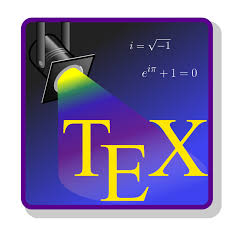
\includegraphics[scale=0.3]{texstudio}
	\caption{TexStudio, editor de \LaTeX.}
	\label{fig:texstudio}
\end{figure}

\subsection{Microsoft Office Word}
Editor de documentos de textos dentro del paquete de ofimática \textit{Microsoft Office}.
\subsection{Libre Office Writer}
Editor de documentos de texto dentro del paquete libre de ofimática \textit{Libre Office}.

\section{Otros}
En este apartado voy a comentar otras herramientas usadas en el proyecto, pero que no entran en ninguno de los apartados anteriores.
\begin{itemize}
	\item \textbf{Microsoft Office PowerPoint}: herramienta para realizar presentaciones, dentro del paquete de ofimática de \textit{Microsoft Office}.
	\item \textbf{Audacity}: programa para el tratado de audios, donde podemos ver las distintas representaciones de la onda y espectrogramas en las distintas escalas.
	\item \textbf{noWifi}: aplicación que permite a la tarjeta de red de un ordenador hacer las funciones de router para desplegar de forma sencilla una red hosteada.
	\item \textbf{RandomKeyGen}: página web que nos permite generar claves aleatorias de distintos tamaños, \url{https://randomkeygen.com/}.
	\item \textbf{Paint}: herramienta para la edición de imágenes.
	\item \textbf{Gimp 2}: herramienta para la edición de imágenes.
	\item \textbf{AZ Screen Recorder}: aplicación móvil que nos permite grabar la pantalla de nuestro dispositivo.
	\item \textbf{GitHub}: control de repisotorios \textit{Git}.
	\item \textbf{ZenHub}: herramienta enlazada con \textit{GitHub} para el control de versiones y técnica \textit{SCRUM}.
\end{itemize}